\documentclass[11pt]{beamer}
\usepackage[utf8]{inputenc}
\usepackage[T1]{fontenc}
\usepackage{amsmath,amssymb}
\usepackage{amsfonts}
\usepackage{paralist}
\usepackage{color}
\usepackage{graphicx}
\usepackage{pgfplots}
\usepackage{authblk}
\usepackage{url}
\usepackage{multirow}
\usepackage{booktabs}
\usepackage{blindtext}
\usepackage{adjustbox}
\usepackage{subcaption}

\mode<presentation> {
	\usetheme{Berlin}
	\usecolortheme{default}}

\title{Final HPC Assigment}
\author{Valentinis Alessio}
\institute{Università degli Studi di Trieste}
\date{27th february 2024}


\begin{document}

\begin{frame}
	\maketitle
\end{frame}

\section{Exercise 1}
\begin{frame}{Exercise 1}
	The goal of the exercise was to estimate the latency of two OpenMPI collective operation, one of which being \textit{Broadcast}. My work focussed on studying
	\begin{itemize}
		\item Broadcast\\
		\item Barrier
	\end{itemize}
	All of these algorithms were studied varying between four implementations, and varying process allocation between \textit{core}, \textit{socket} and \textit{node}.
\end{frame}

\begin{frame}{Broadcast}
	I've studied four different implementation of the algorithm:
	\begin{itemize}
		\item Default
		\item Basic Linear
		\item Chain
		\item Binary tree
	\end{itemize}
	Having many degrees of freedom to analyze, I've decided to sequentially fix some of them, in order to see the impact of few on the \textit{Avg Latency} variable.
\end{frame}

\begin{frame}{Fixing message size of 1 Byte}
	
	\begin{figure}[h]
		\centering
		\begin{subfigure}{0.45\textwidth}
			\centering
			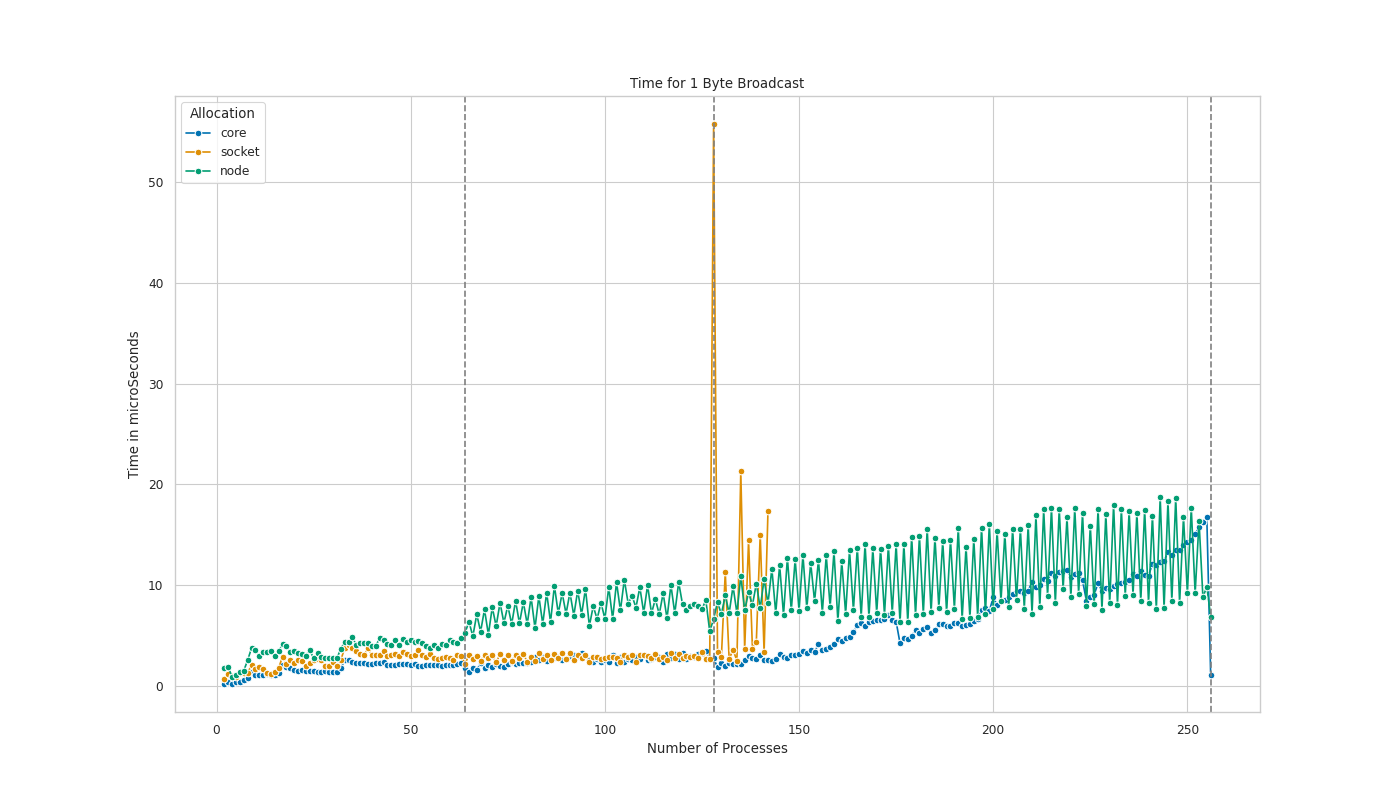
\includegraphics[width=0.7\linewidth]{../exercise1/plots/bcast_default_1byte}
			\caption{Average Latency vs n. processes in default algorithm}
			\label{fig:bcastdefault1byte}
		\end{subfigure}
		\begin{subfigure}{0.45\textwidth}
			\centering
			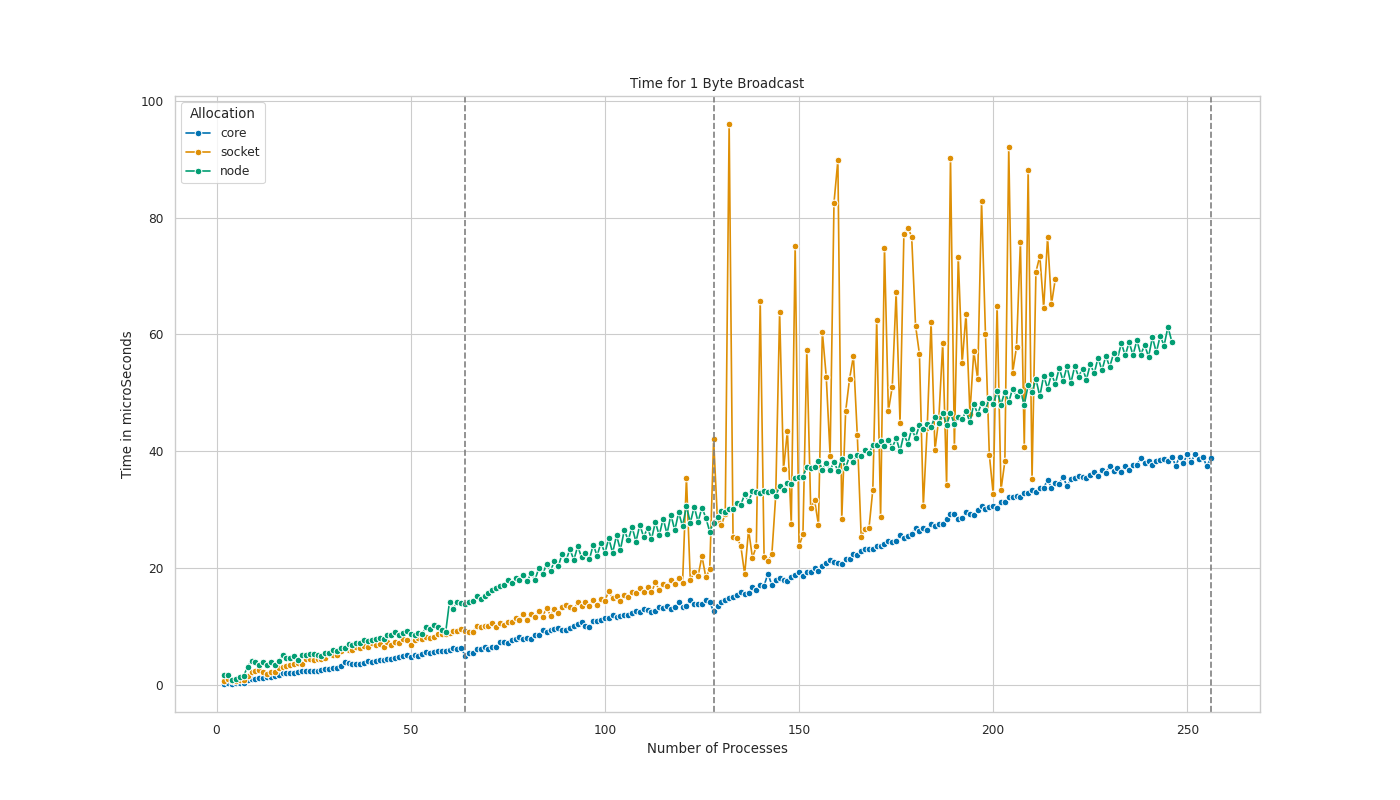
\includegraphics[width=0.7\linewidth]{../exercise1/plots/bcast_linear_1byte}
			\caption{Average Latency vs n. processes in linear algorithm}
			\label{fig:bcastlinear1byte}
		\end{subfigure}
		\begin{subfigure}{0.45\textwidth}
			\centering
			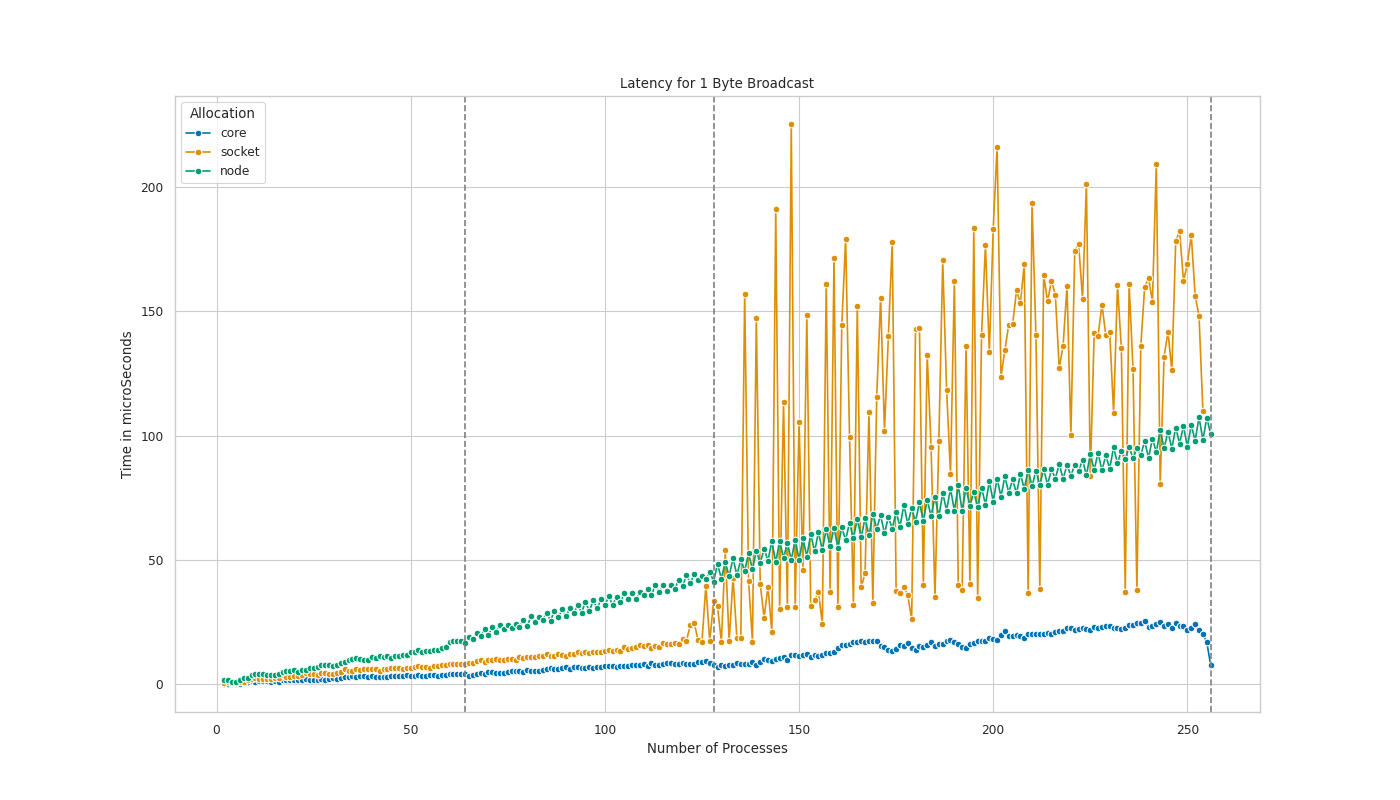
\includegraphics[width=0.7\linewidth]{../exercise1/plots/bcast_chain_1byte}
			\caption{Average Latency vs n. processes in chain algorithm}
			\label{fig:bcastchain1byte}
		\end{subfigure}
		\begin{subfigure}{0.45\textwidth}
			\centering
			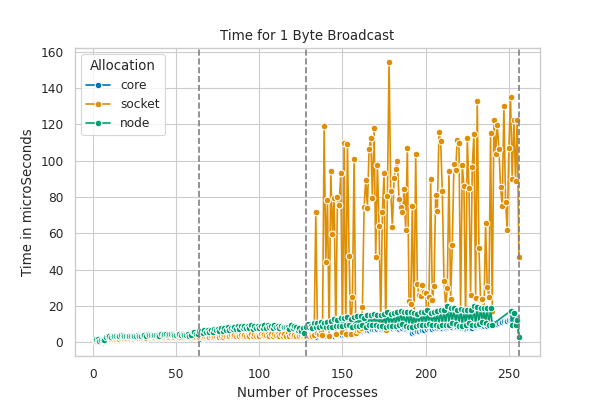
\includegraphics[width=0.7\linewidth]{../exercise1/plots/bcast_bintree_1byte}
			\caption{Average Latency vs n. processes in binary tree algorithm}
			\label{fig:bcastbintree1byte}
		\end{subfigure}
	\end{figure}
\end{frame}

\begin{frame}{Fixing \textit{core} allocation and varying message size}
	\begin{figure}[h]
		\centering
		\begin{subfigure}{0.45\textwidth}
			\centering
			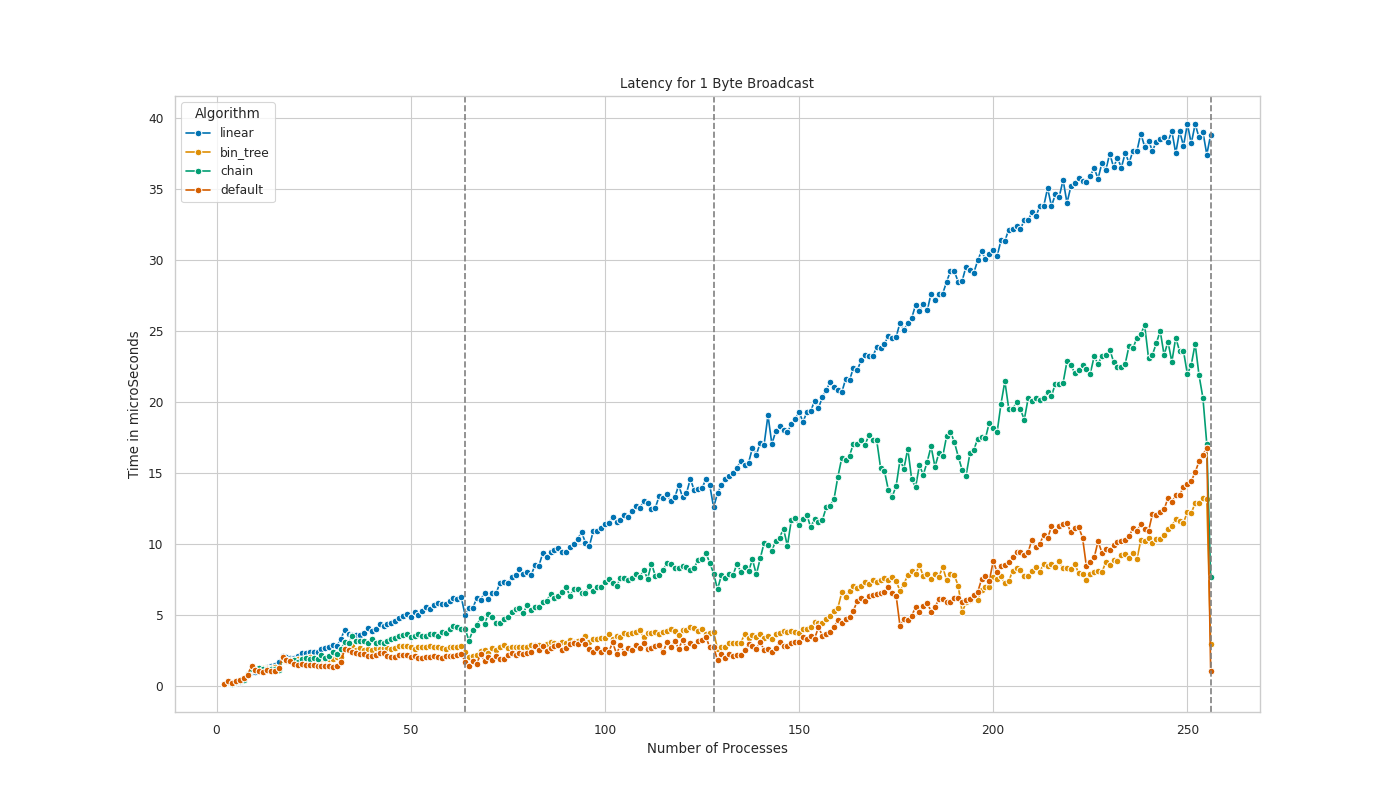
\includegraphics[width=0.7\linewidth]{../exercise1/plots/bcast_all_1byte}
			\caption{Latency vs n. processes by algorithm}
			\label{fig:bcastall1byte}
		\end{subfigure}
		\begin{subfigure}{0.45\textwidth}
			\centering
			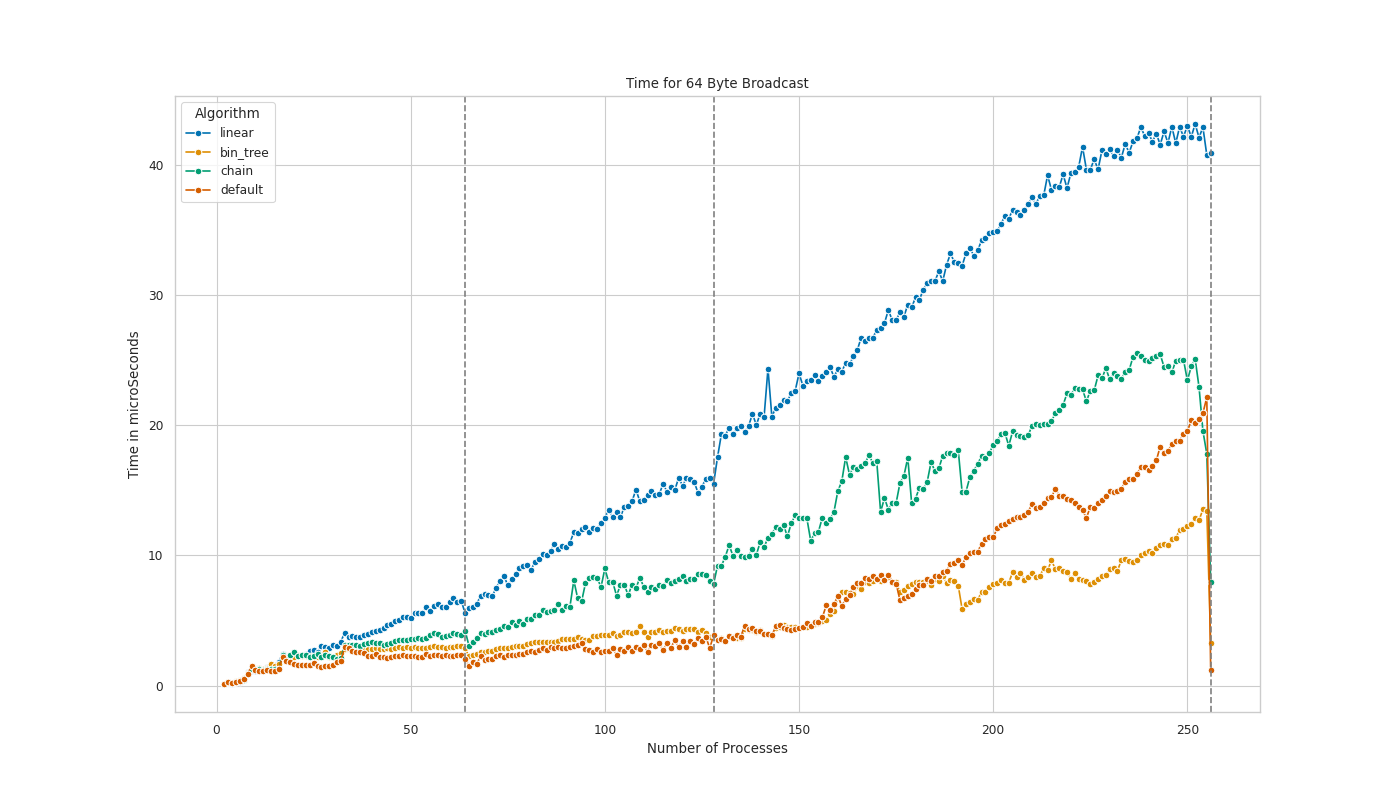
\includegraphics[width=0.7\linewidth]{../exercise1/plots/bcast_all_64byte}
			\caption{Average Latency vs n. processes for 64 byte message}
			\label{fig:bcastall64byte}
		\end{subfigure}
		\begin{subfigure}{0.45\textwidth}
			\centering
			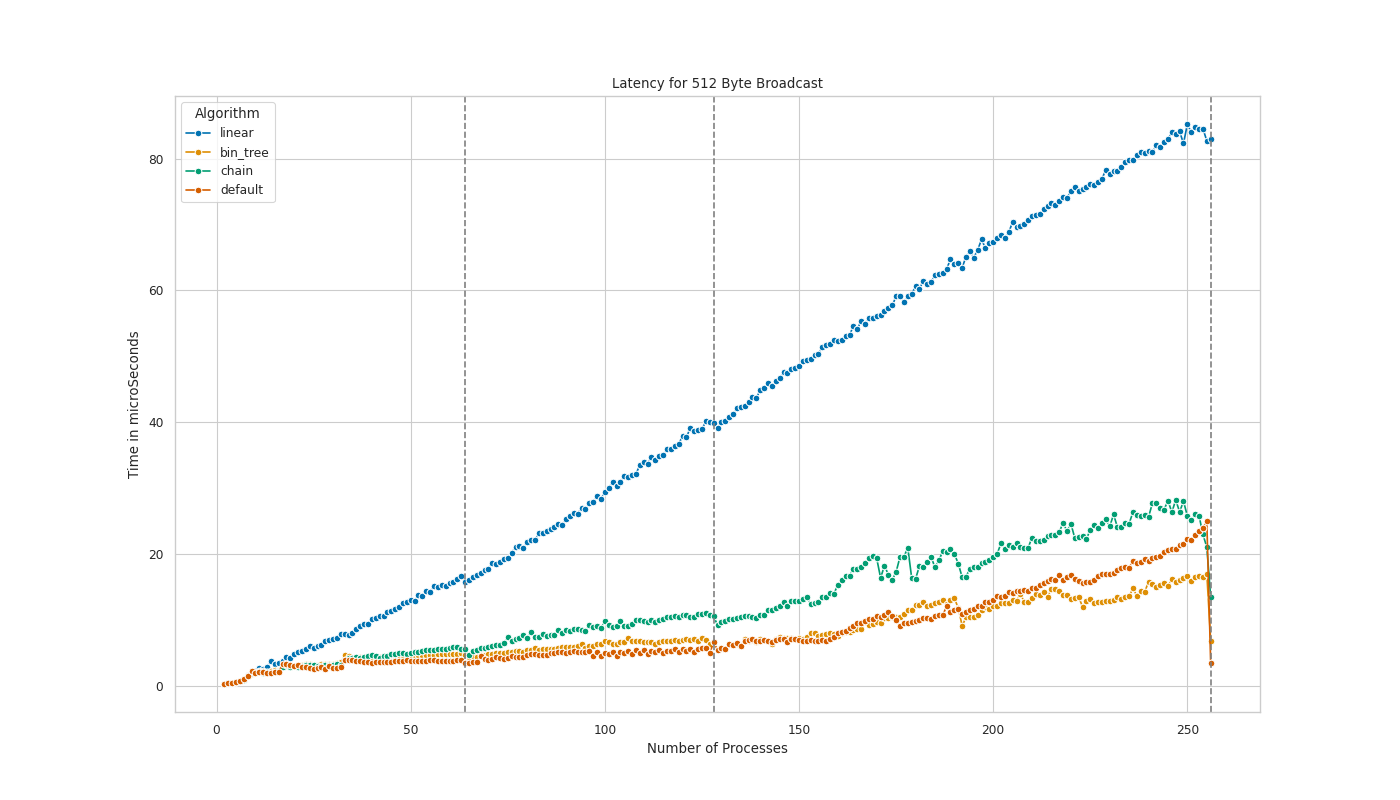
\includegraphics[width=0.7\linewidth]{../exercise1/plots/bcast_all_512byte}
			\caption{Average Latency vs n. processes in 512 byte message}
			\label{fig:bcastall512byte}
		\end{subfigure}
		\begin{subfigure}{0.45\textwidth}
			\centering
			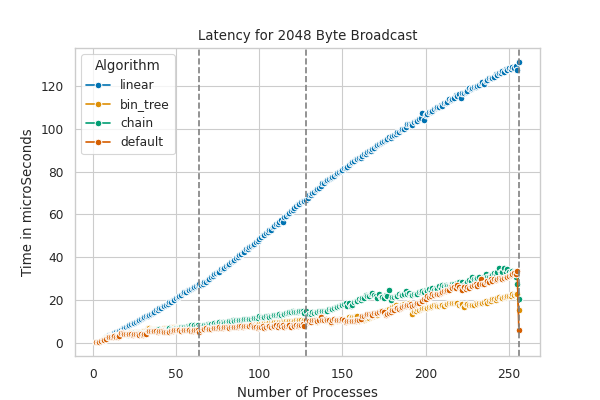
\includegraphics[width=0.7\linewidth]{../exercise1/plots/bcast_all_2048byte}
			\caption{Average Latency vs n. processes in 2024 byte message}
			\label{fig:bcastall2048byte}
		\end{subfigure}
	\end{figure}
\end{frame}

\begin{frame}{Model}
	\begin{center}
		% latex table generated in R 4.3.1 by xtable 1.8-4 package
% Wed Feb 14 17:42:34 2024
\begin{tabular}{rrrrr}
  \hline
 & Estimate & Std. Error & t value & Pr($>$$|$t$|$) \\ 
  \hline
(Intercept) & -68.0031 & 5.0067 & -13.58 & 0.0000 \\ 
  Algorithmchain & 48.3330 & 4.5653 & 10.59 & 0.0000 \\ 
  Algorithmdefault & 4.7424 & 4.5774 & 1.04 & 0.3002 \\ 
  Algorithmlinear & 12.0579 & 4.6361 & 2.60 & 0.0093 \\ 
  Allocationnode & 39.0153 & 3.9529 & 9.87 & 0.0000 \\ 
  Allocationsocket & 63.3617 & 3.9943 & 15.86 & 0.0000 \\ 
  Processes & 0.5054 & 0.0225 & 22.49 & 0.0000 \\ 
  MessageSize & 0.0013 & 0.0027 & 0.46 & 0.6452 \\ 
   \hline
\end{tabular}

	\end{center}
	Model analysis with all variable included %($R^2 = 2\%$)
\end{frame}
\begin{frame}
	\begin{center}
		% latex table generated in R 4.3.1 by xtable 1.8-4 package
% Wed Feb 14 18:00:32 2024
\begin{tabular}{rrrrr}
  \hline
 & Estimate & Std. Error & t value & Pr($>$$|$t$|$) \\ 
  \hline
(Intercept) & -11.7242 & 0.2489 & -47.10 & 0.0000 \\ 
  Algorithmchain & 5.3313 & 0.2587 & 20.60 & 0.0000 \\ 
  Algorithmdefault & 0.5461 & 0.2587 & 2.11 & 0.0348 \\ 
  Algorithmlinear & 23.9312 & 0.2587 & 92.49 & 0.0000 \\ 
  Processes & 0.1198 & 0.0012 & 96.41 & 0.0000 \\ 
  MessageSize & 0.0080 & 0.0002 & 51.66 & 0.0000 \\ 
   \hline
\end{tabular}

	\end{center}
	Model analysis with fixed allocation %($R^2 = 65\%$)
\end{frame}

\begin{frame}{Barrier}
	Also here I've analyzed four different implementations:
	\begin{itemize}
		\item Default
		\item Linear
		\item Double Ring
		\item Bruck algorithm
	\end{itemize}
	The same analysis steps of the previous algorithm apply
\end{frame}

\begin{frame}{Vary allocation}
	\begin{figure}[h]
		\centering
		\begin{subfigure}{0.45\textwidth}
			\centering
			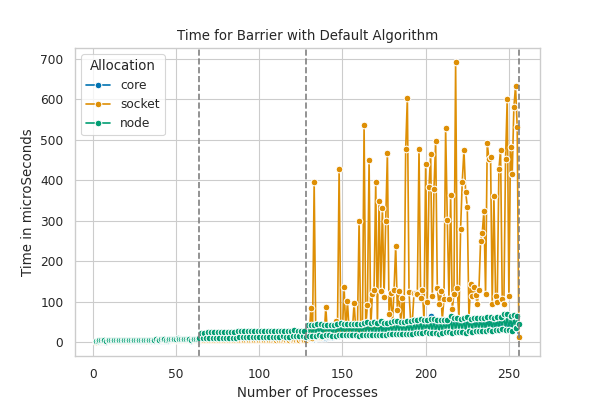
\includegraphics[width=0.7\linewidth]{../exercise1/plots/barrier_default}
			\caption{Average Latency vs n. processes in default algorithm}
			\label{fig:barrierdefault}
		\end{subfigure}
		\begin{subfigure}{0.45\textwidth}
			\centering
			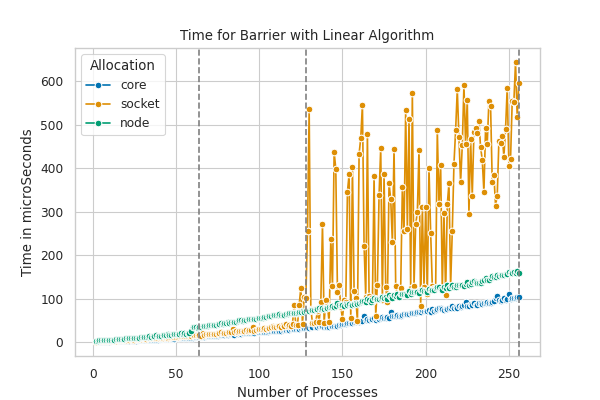
\includegraphics[width=0.7\linewidth]{../exercise1/plots/barrier_linear}
			\caption{Average Latency vs n. processes in linear algorithm}
			\label{fig:barrierlinear}
		\end{subfigure}
		\begin{subfigure}{0.45\textwidth}
			\centering
			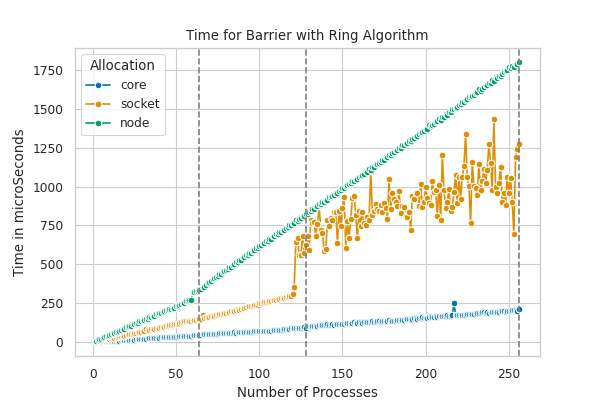
\includegraphics[width=0.7\linewidth]{../exercise1/plots/barrier_ring}
			\caption{Average Latency vs n. processes in double ring algorithm}
			\label{fig:barrierring}
		\end{subfigure}
		\begin{subfigure}{0.45\textwidth}
			\centering
			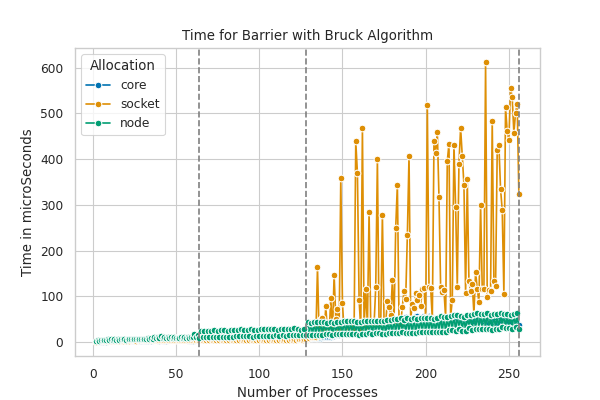
\includegraphics[width=0.7\linewidth]{../exercise1/plots/barrier_bruck}
			\caption{Average Latency vs n. processes in bruck algorithm}
			\label{fig:barrierbruck}
		\end{subfigure}
	\end{figure}
\end{frame}

\begin{frame}{Fixing Allocation}
	\begin{figure}[h]
		\centering
		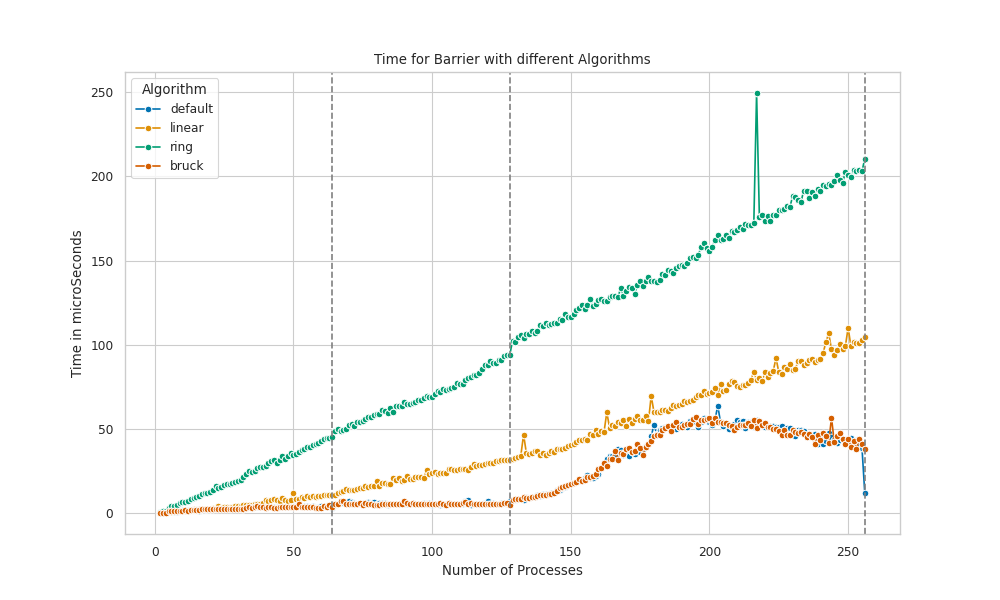
\includegraphics[width=0.7\linewidth]{../exercise1/plots/barrier_core}
		\caption{Latency vs n. processes by algorithm}
		\label{fig:barriercore}
	\end{figure}
\end{frame}

\begin{frame}{Performance Model}
	\begin{center}
		% latex table generated in R 4.3.1 by xtable 1.8-4 package
% Wed Feb 14 17:58:54 2024
\begin{tabular}{rrrrr}
  \hline
 & Estimate & Std. Error & t value & Pr($>$$|$t$|$) \\ 
  \hline
(Intercept) & -68.0031 & 5.0067 & -13.58 & 0.0000 \\ 
  Algorithmchain & 48.3330 & 4.5653 & 10.59 & 0.0000 \\ 
  Algorithmdefault & 4.7424 & 4.5774 & 1.04 & 0.3002 \\ 
  Algorithmlinear & 12.0579 & 4.6361 & 2.60 & 0.0093 \\ 
  Allocationnode & 39.0153 & 3.9529 & 9.87 & 0.0000 \\ 
  Allocationsocket & 63.3617 & 3.9943 & 15.86 & 0.0000 \\ 
  Processes & 0.5054 & 0.0225 & 22.49 & 0.0000 \\ 
  MessageSize & 0.0013 & 0.0027 & 0.46 & 0.6452 \\ 
   \hline
\end{tabular}

	\end{center}
	Model with all parameters %($R^2 = 55\%$)
\end{frame}

\begin{frame}
	\begin{center}
		% latex table generated in R 4.3.1 by xtable 1.8-4 package
% Wed Feb 14 18:00:38 2024
\begin{tabular}{rrrrr}
  \hline
 & Estimate & Std. Error & t value & Pr($>$$|$t$|$) \\ 
  \hline
(Intercept) & -34.3959 & 1.5941 & -21.58 & 0.0000 \\ 
  Algorithmdefault & 0.0435 & 1.6956 & 0.03 & 0.9795 \\ 
  Algorithmlinear & 19.0073 & 1.6956 & 11.21 & 0.0000 \\ 
  Algorithmring & 78.4787 & 1.6956 & 46.28 & 0.0000 \\ 
  Processes & 0.4335 & 0.0081 & 53.23 & 0.0000 \\ 
   \hline
\end{tabular}

	\end{center}
	Model with fixed allocation %($R^2 = 80\%$)
\end{frame}

\section{Exercise 2b}
\begin{frame}{Exercise 2b}
	The aim of the exercise was to implement a parallel version of the Quicksort routine through the use of both OpenMP and MPI, analyzing its Scalability and performance.
\end{frame}

\begin{frame}
	\begin{figure}[h]
		\centering
		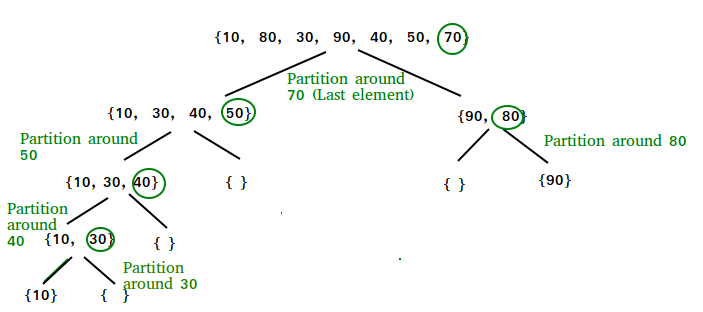
\includegraphics[width=0.7\linewidth]{../report/QuickSort2}
		\caption[Illustration of Quicksort algorithm]{}
		\label{fig:quicksort2}
	\end{figure}
\end{frame}

\begin{frame}
	\begin{figure}[h]
		\centering
		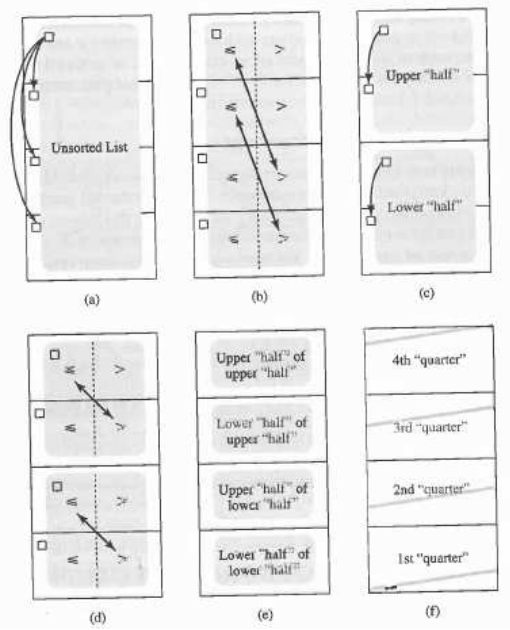
\includegraphics[height=0.7\linewidth]{../report/Parallel_quicksort}
		\caption{Sketch of parallel quicksort}
		\label{fig:parallelquicksort}
	\end{figure}
\end{frame}

\begin{frame}{OpenMP scalability}
	\begin{figure}[h]
		\centering
		\begin{subfigure}{0.75\textwidth}
			\centering
			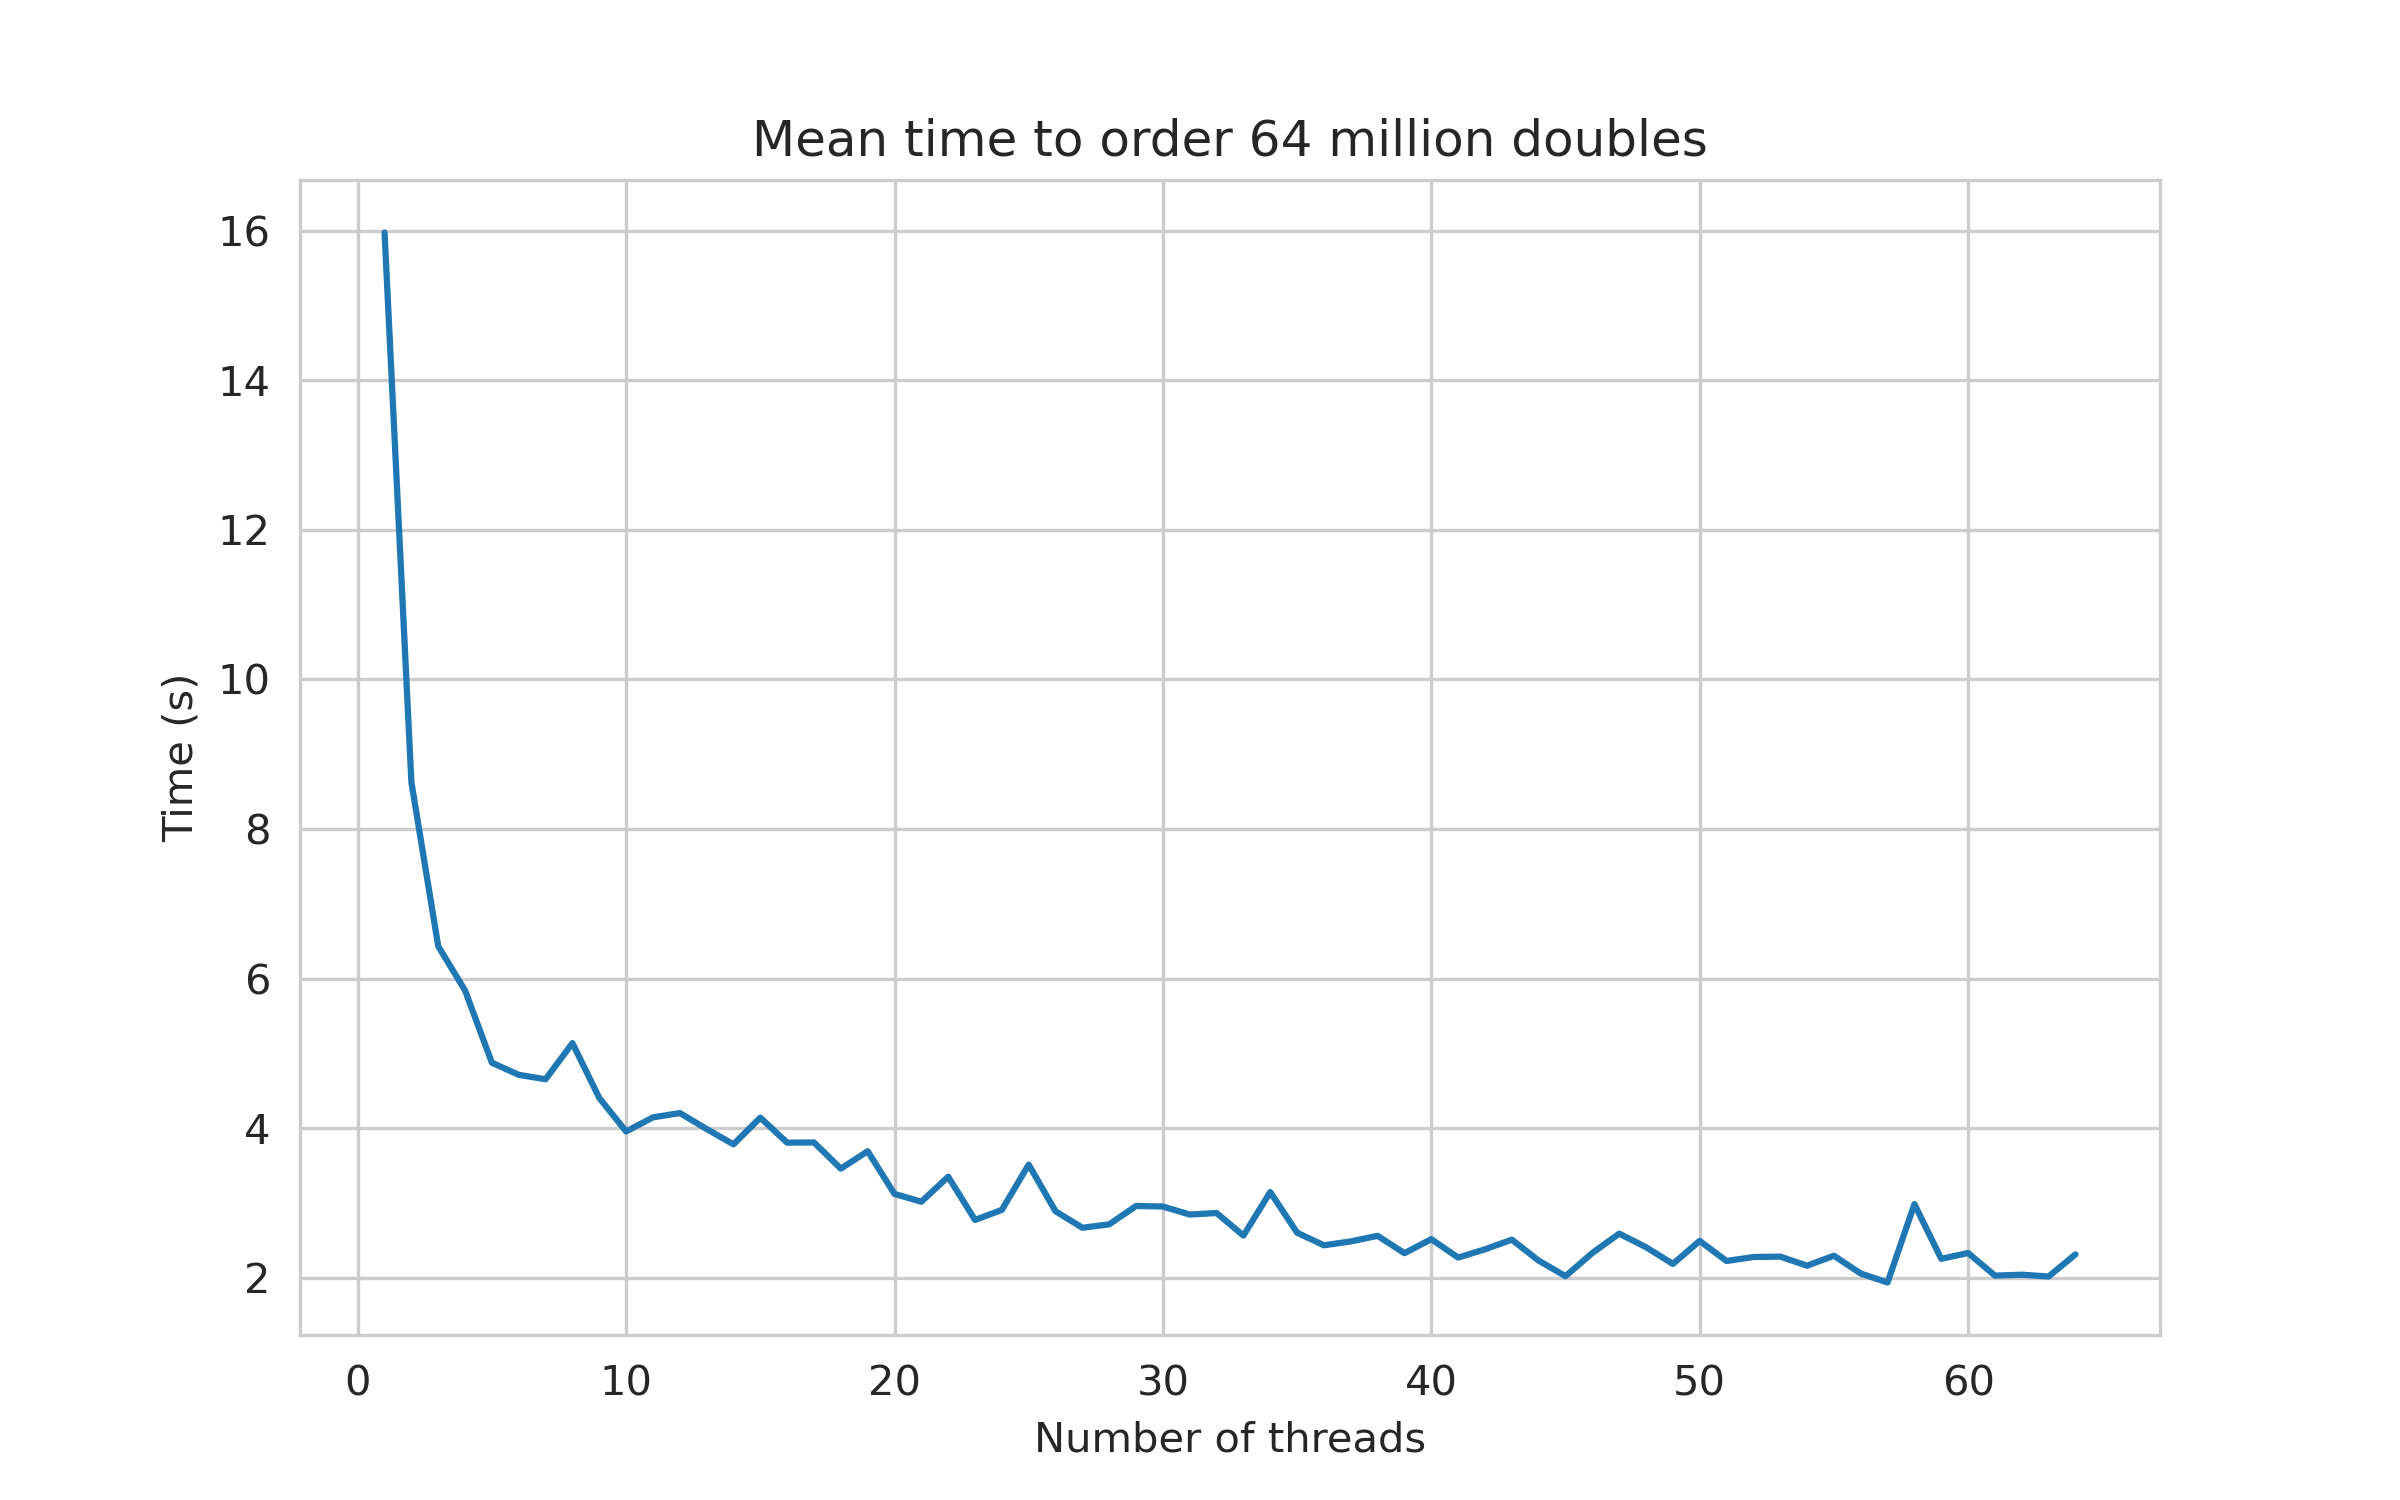
\includegraphics[width=0.5\linewidth]{../exercise2/plots/omp_timings}
			\label{fig:omptimings}
		\end{subfigure}
		\begin{subfigure}{0.75\textwidth}
			\centering
			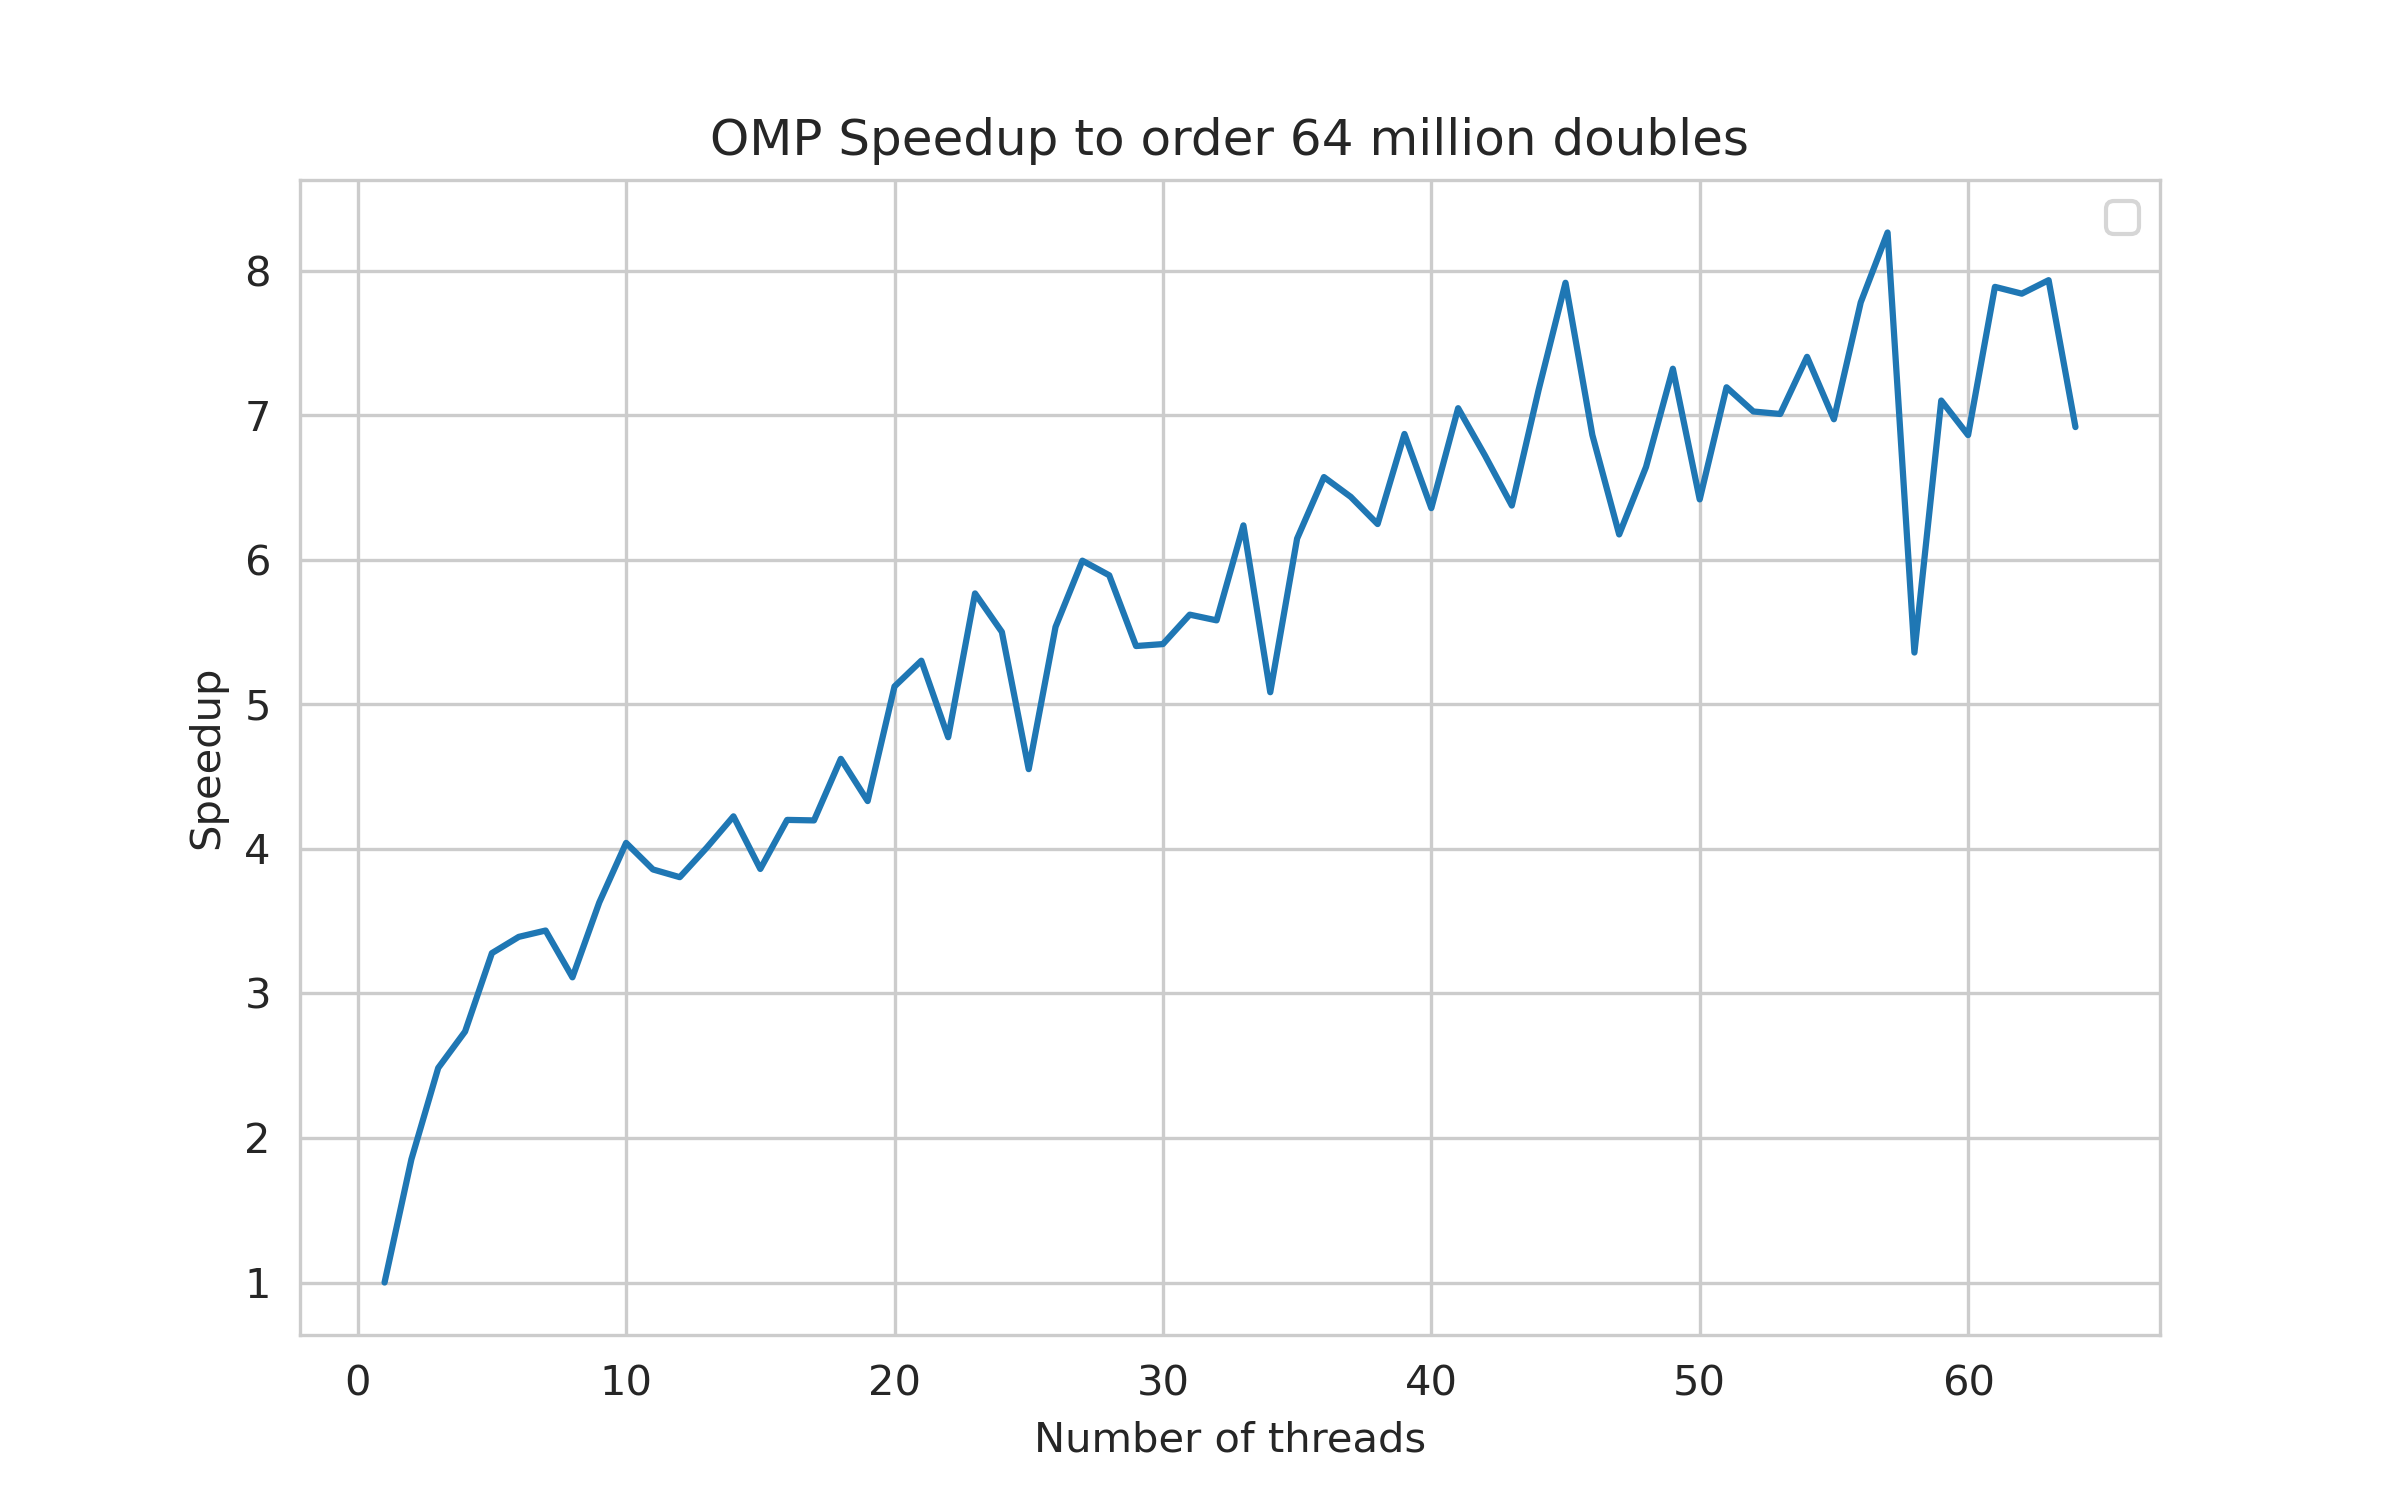
\includegraphics[width=0.7\linewidth]{../exercise2/plots/omp_speedup}
			\label{fig:ompspeedup}
		\end{subfigure}
	\end{figure}
\end{frame}

\begin{frame}{Strong MPI scalability}
	\begin{figure}
		\begin{subfigure}{0.75\textwidth}
			\centering
			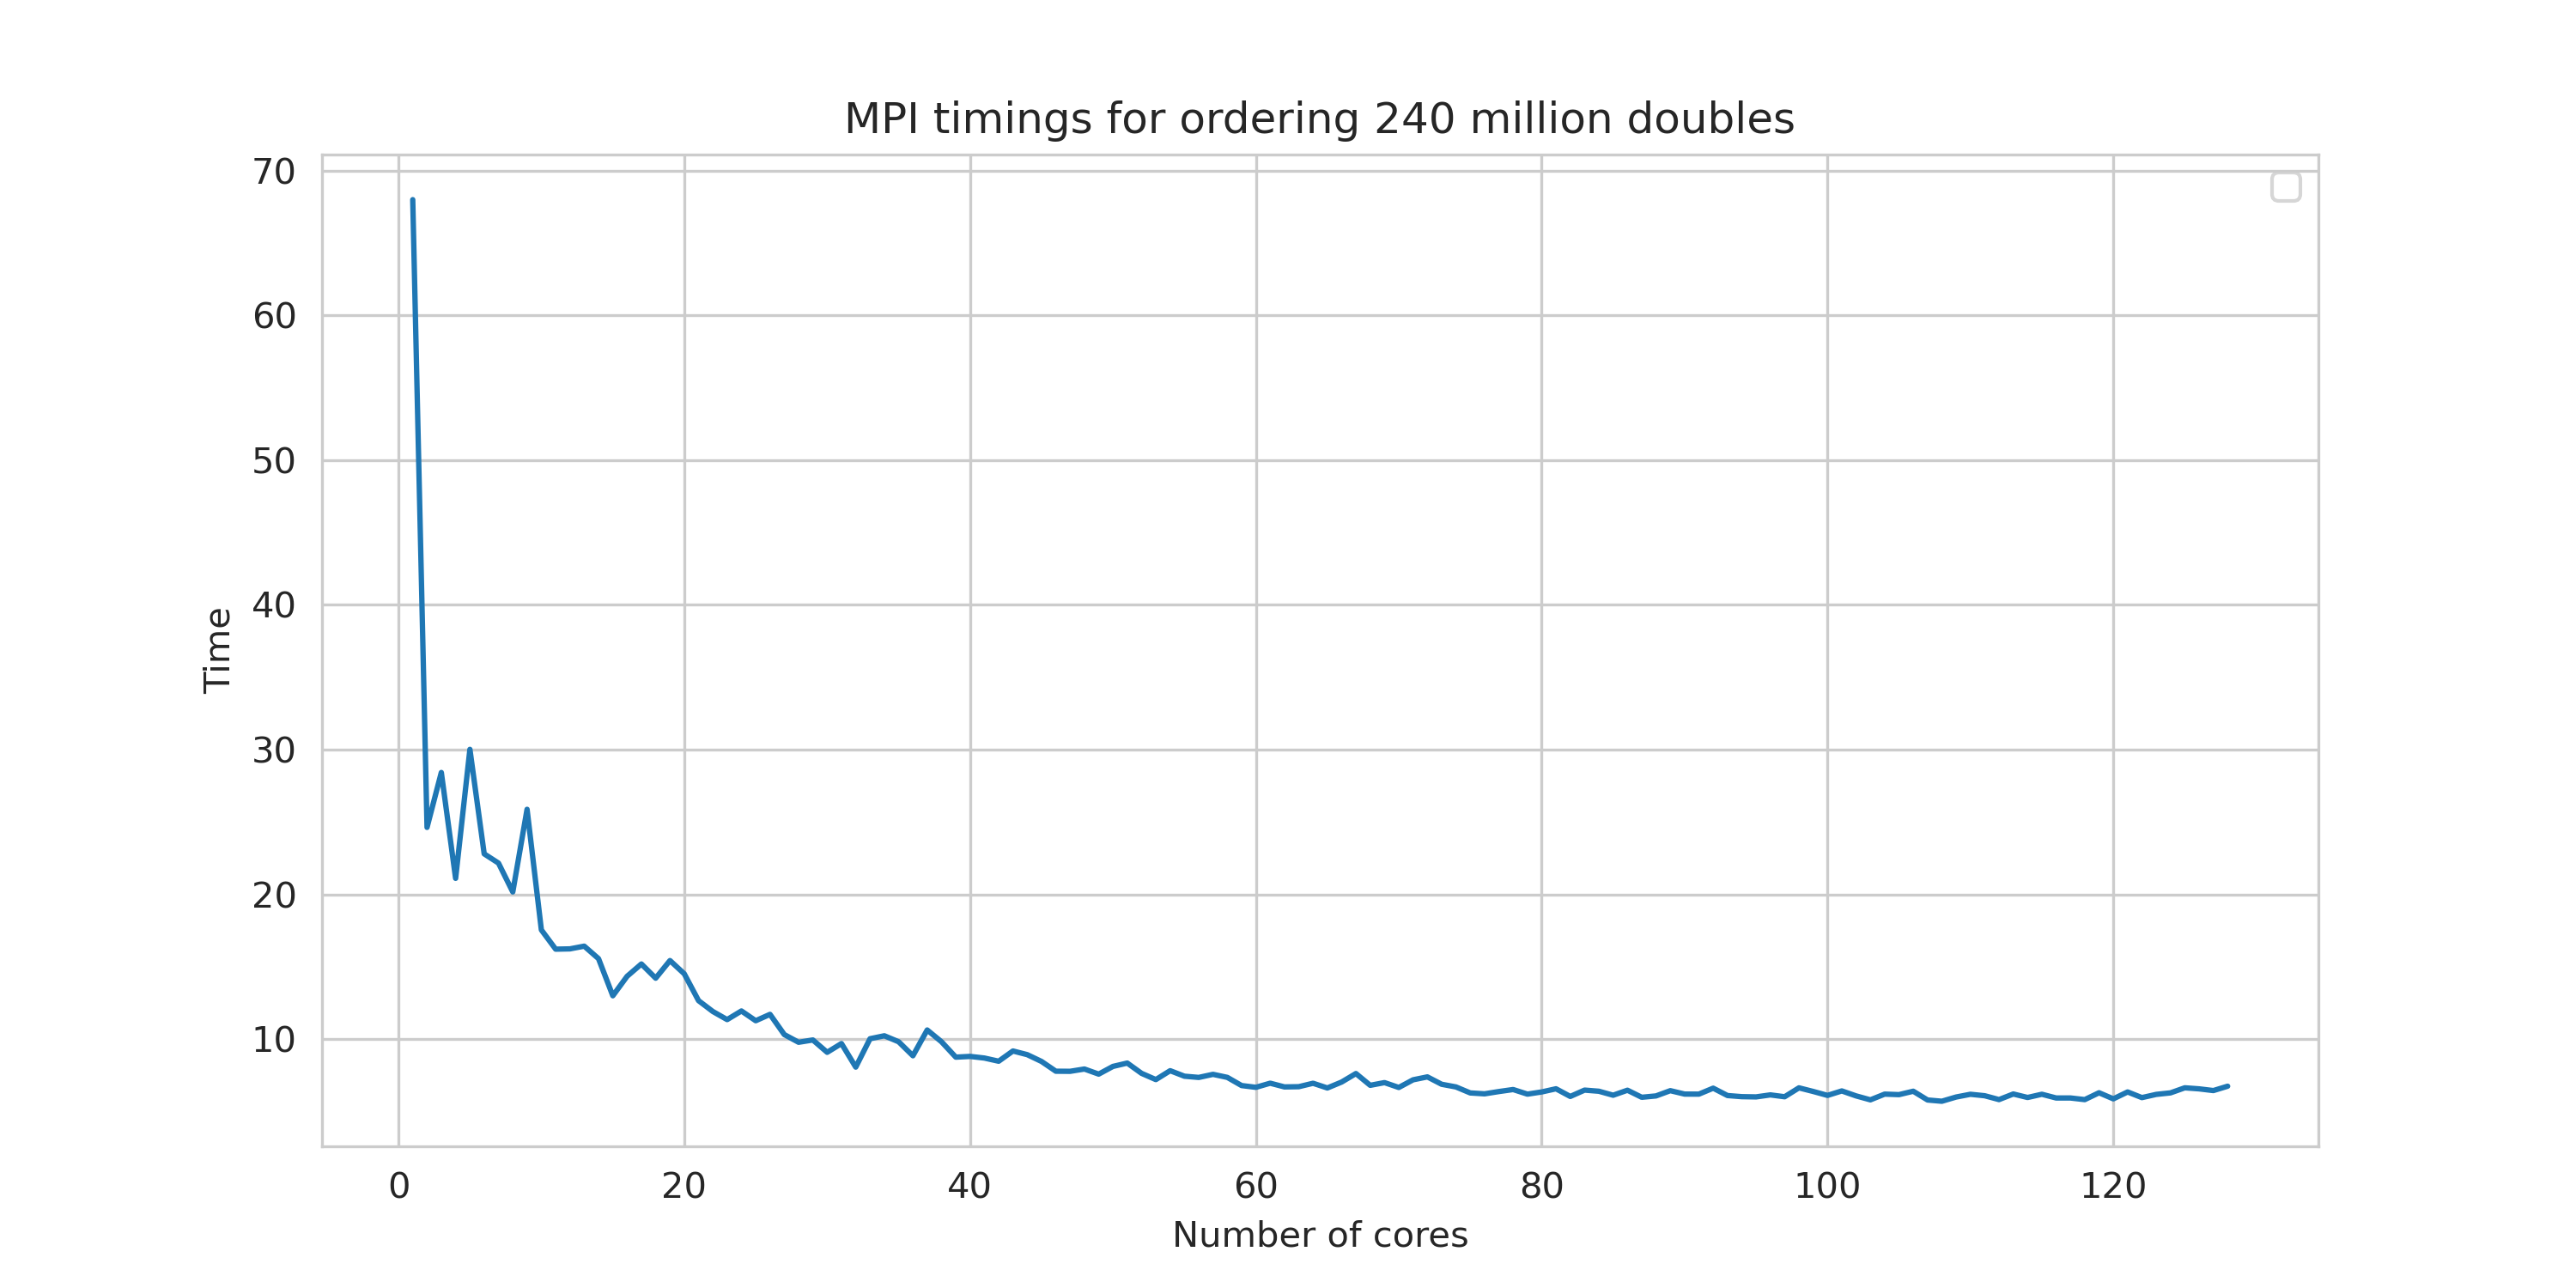
\includegraphics[width=0.7\linewidth]{../exercise2/plots/smpi_timings}
			\label{fig:smpitimings}
		\end{subfigure}
		\begin{subfigure}{0.75\textwidth}
			\centering
			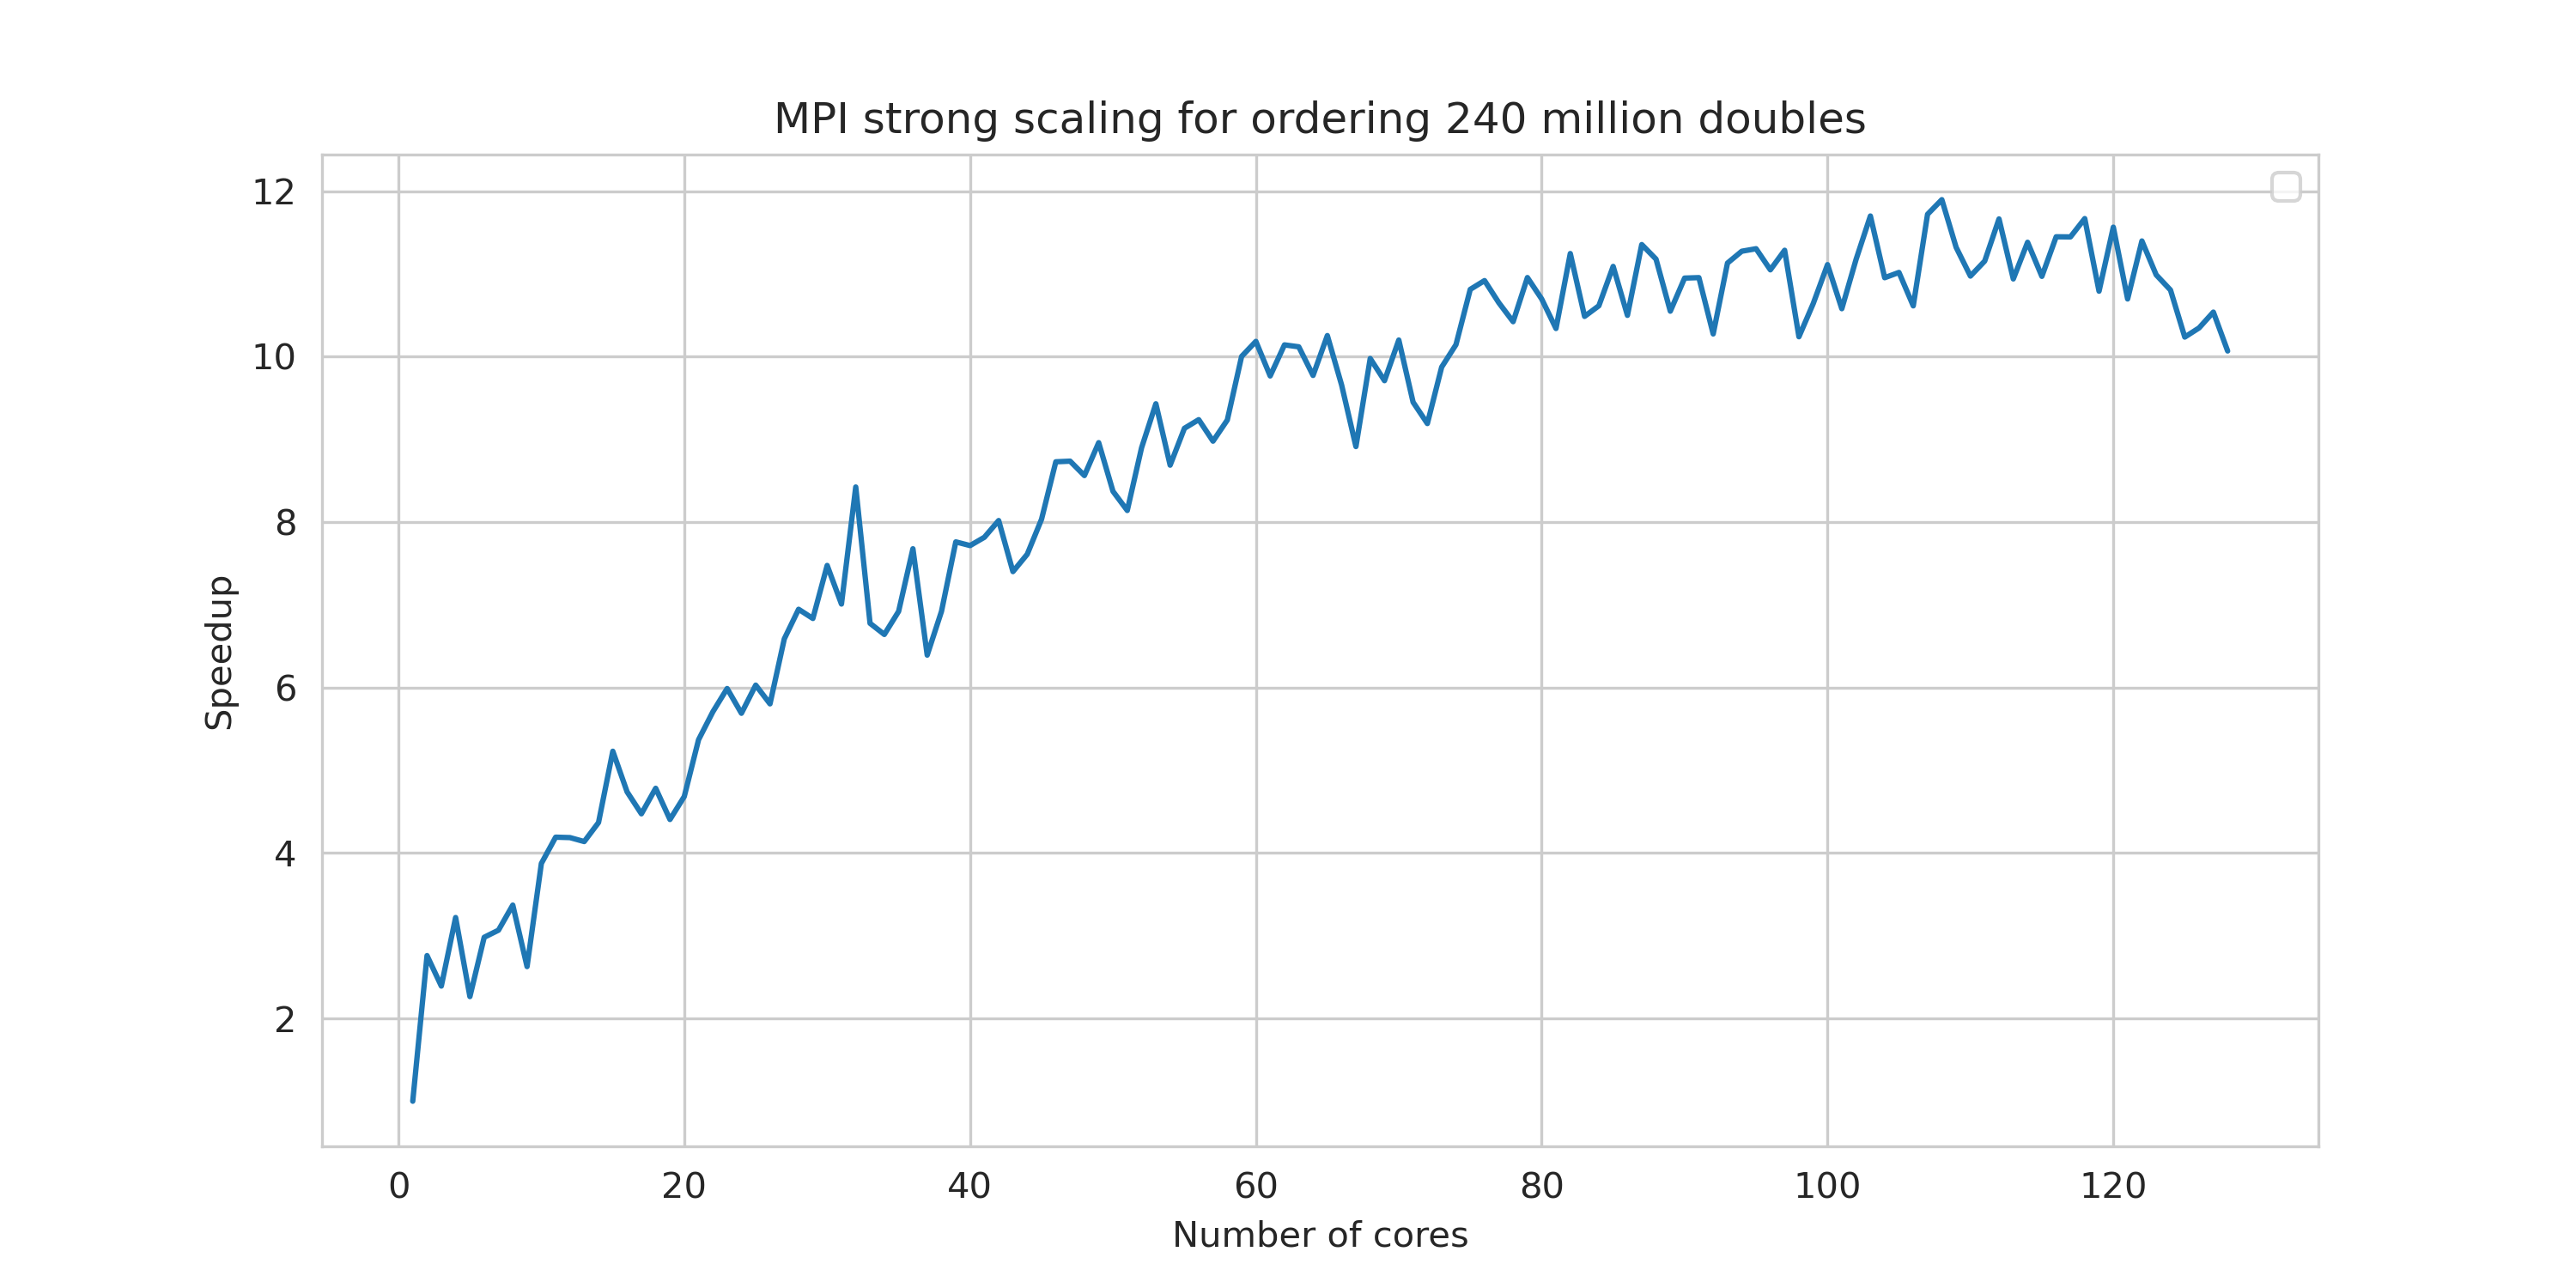
\includegraphics[width=0.7\linewidth]{../exercise2/plots/mpi_scaling}
			\label{fig:mpiscaling}
		\end{subfigure}
	\end{figure}
\end{frame}

\begin{frame}{Weak MPI Scalability}
	\begin{figure}[h]
		\centering
		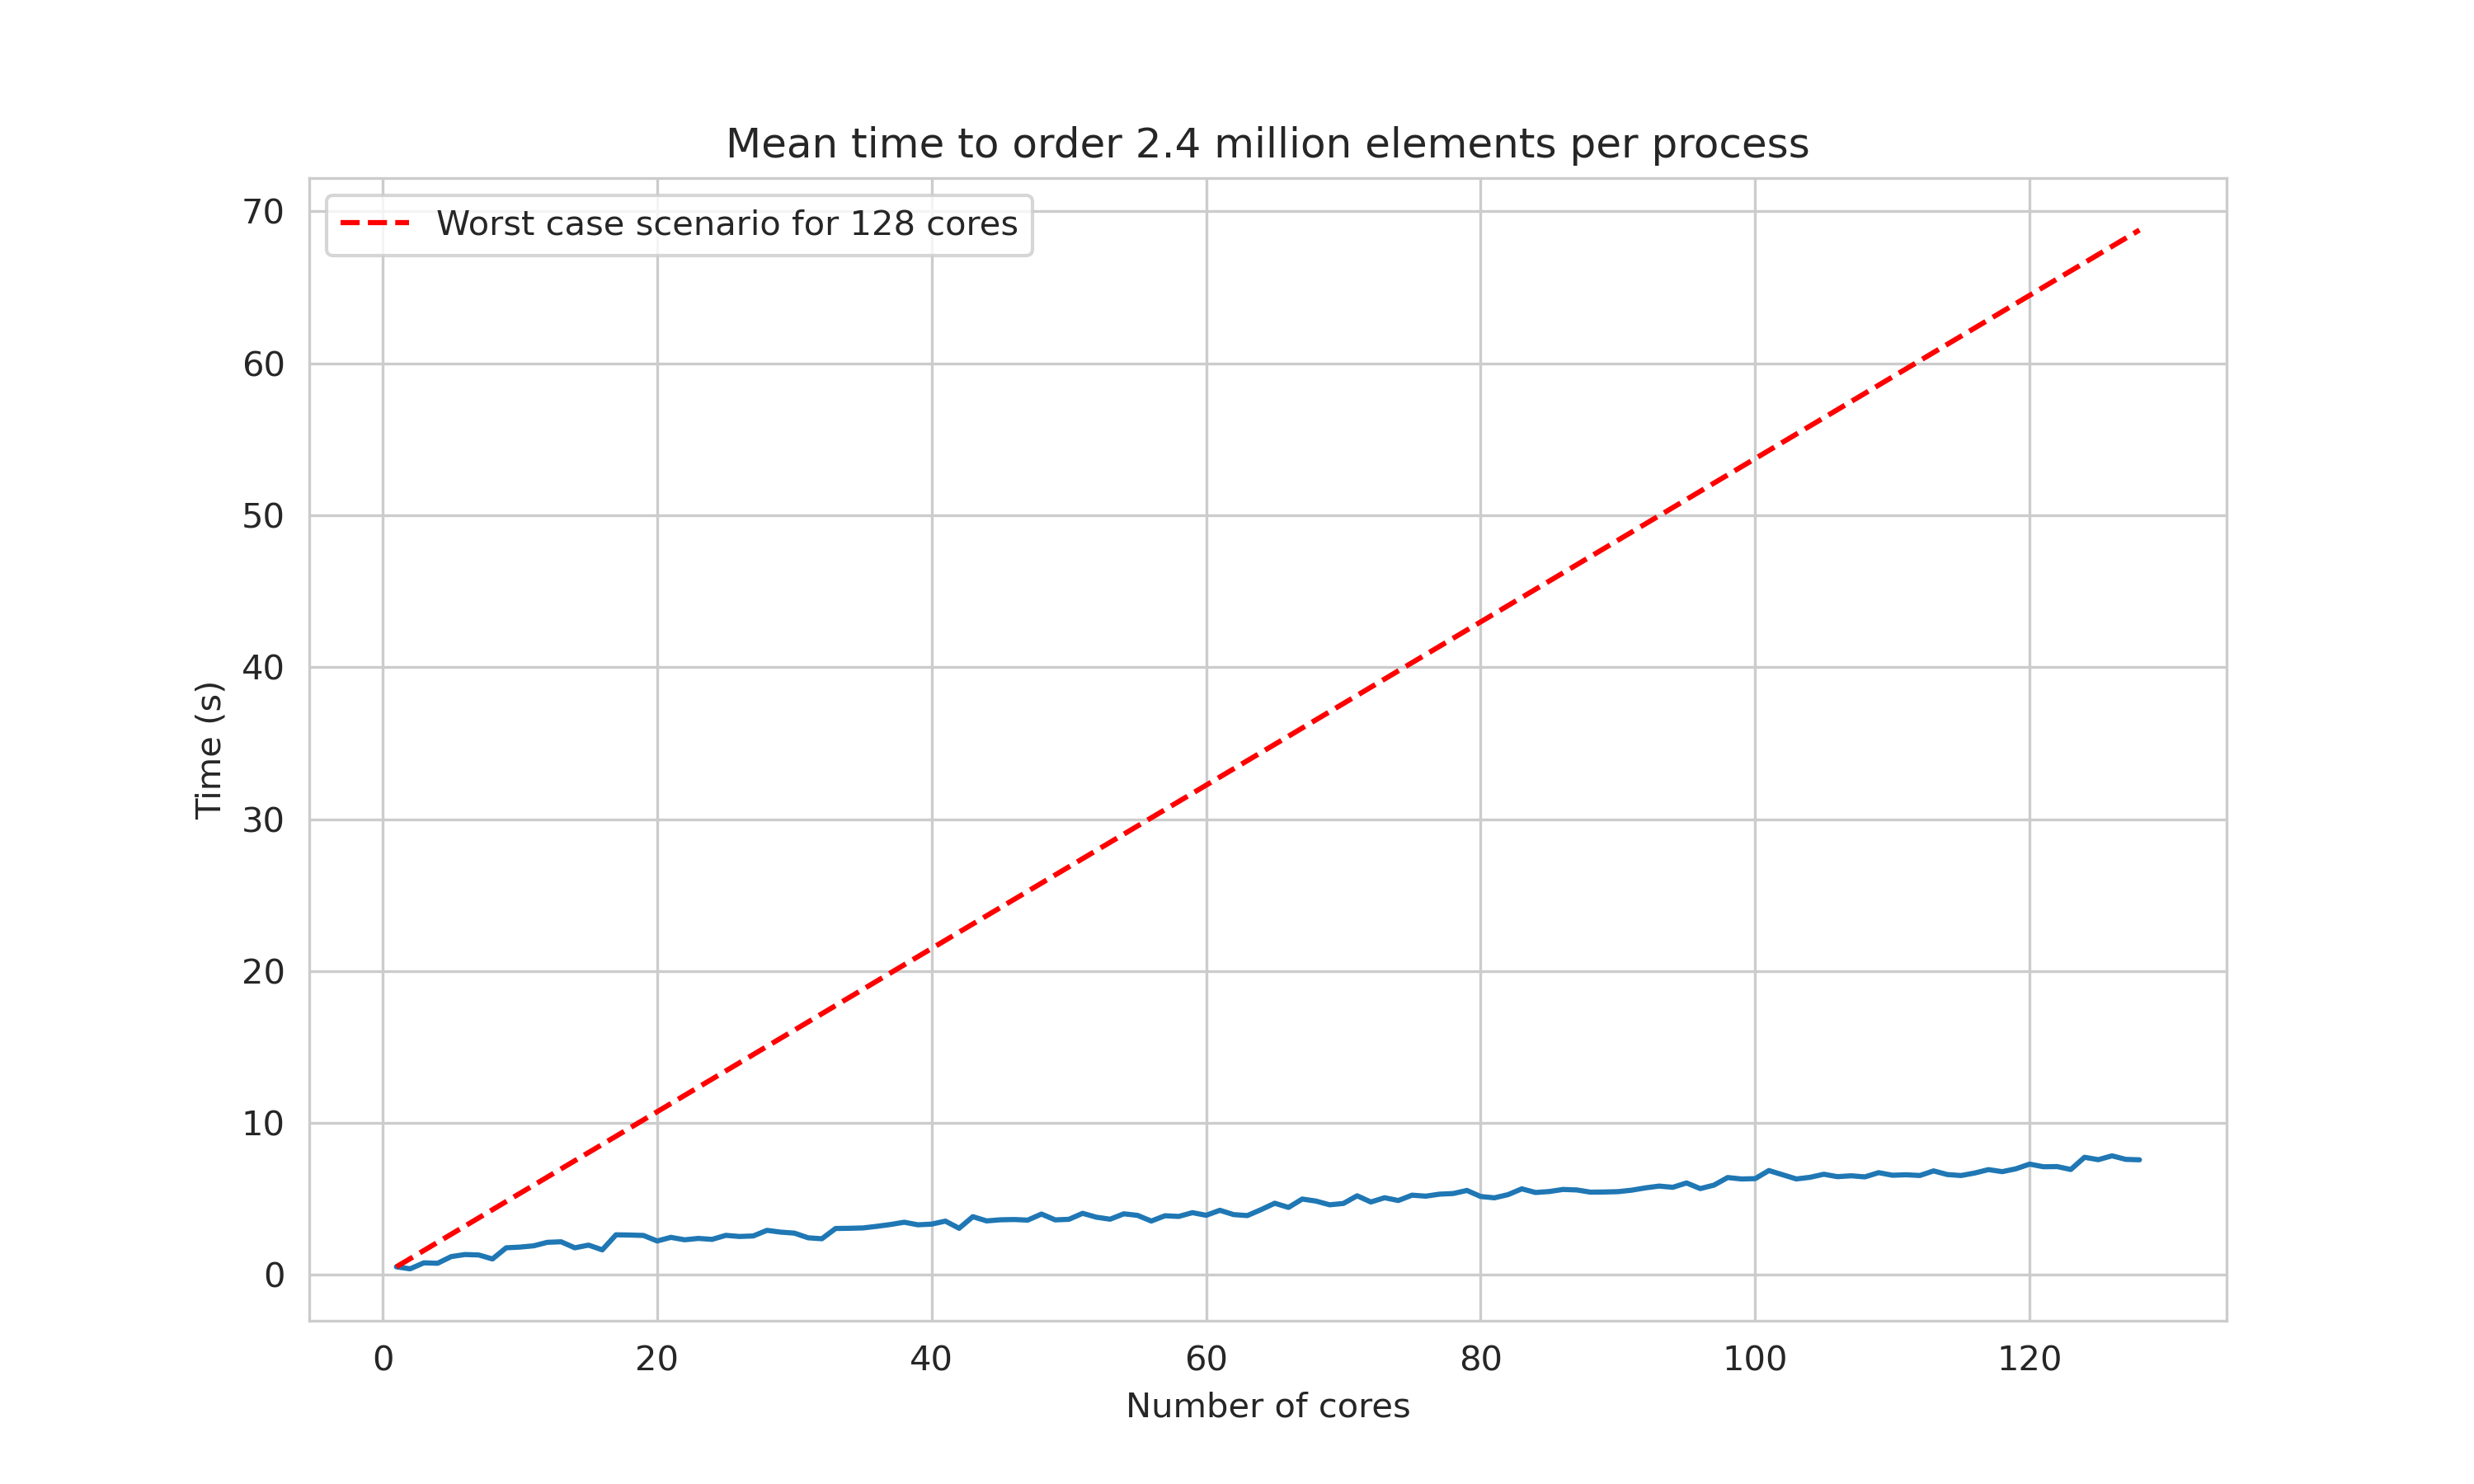
\includegraphics[width=0.7\linewidth]{../exercise2/plots/wmpi_timings}
		\caption[wMPI Timings]{Time vs \#cores at constant workload}
		\label{fig:wmpitimings}
	\end{figure}
\end{frame}

\begin{frame}{Conclusions and Improvement}
	Even though the algorithm doesn't scale linearly, it does what expected, and provides decent results, easing computational time of a very efficient sorting routine as Quicksort.
	
	Possible improvements:
	\begin{itemize}
		\item Try and see if a completely random pivot would work better than selecting a "good" one.
		\item Try and implement an algorithm with a linear number of communications with respect to number of processes
		\item Implement a similar approach also in shared memory
		\item Try a different partitioning routine which could exploit parallelism better
	\end{itemize}
\end{frame}

\end{document}